\begin{vbframe}{}

\vfill

\textbf{}

	\begin{itemize}
		\item 
		\item 
		\item 
	\end{itemize}

\vfill

\end{vbframe}









\begin{vbframe}{Limitation of the Transformer}

\vfill

\begin{figure}
\centering
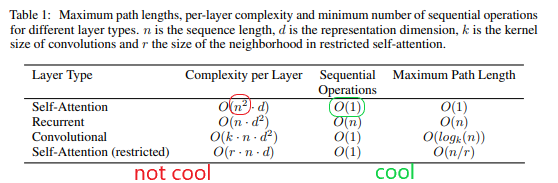
\includegraphics[width = 6.5cm]{figure/n_squared.png}\\ 
\footnotesize{Source:} \href{https://arxiv.org/pdf/1706.03762.pdf}{\footnotesize Vaswani et al. (2017)}
\end{figure}

\textbf{Advantage:}

\begin{itemize}
	\item Every token can \textit{directly} attend to each other token
	\item Cf. RNN: At worst $n$ sequential operations (last to first token)
\end{itemize}

\textbf{Severe Limitation:}

\begin{itemize}
	\item Every token attends to each other token (incl. itself)\\
				$\to$ We need to calculate $n^2$ attention weights
	\item Computational complexity of Transformer scales quadratically with the sequence length\\
				$\to$ Longer sequences are disproportionally expensive
\end{itemize}

\vfill

\end{vbframe}
